\documentclass{article}
\usepackage{geometry}
\geometry{a4paper}
\usepackage{graphicx,subfig}

\begin{document}
	\begin{figure}
		\centering
		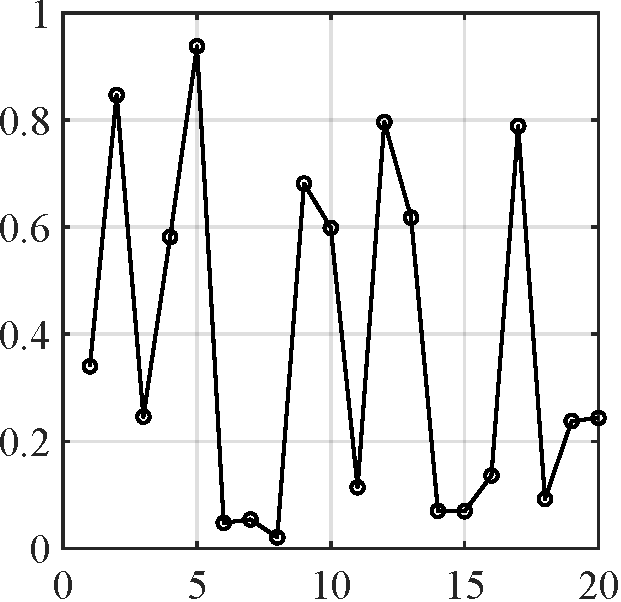
\includegraphics[width=0.2\textwidth]{pic-1.pdf}
		\caption{This is a random data series 1, and here is short caption.}
		\vspace{-30em}
	\end{figure}

	\begin{figure}
		\def\CE{0.20}
		\centering
		\subfloat[]{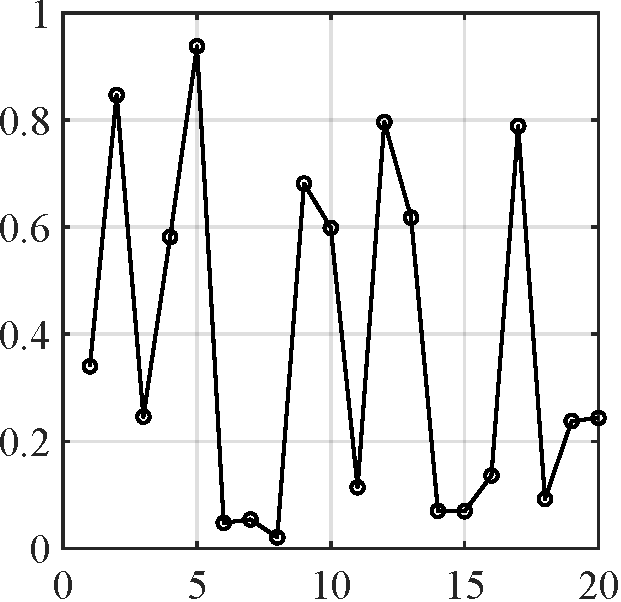
\includegraphics[height=\CE\textwidth,width=\CE\textwidth]{pic-1.pdf}\label{fig-a}}\hfill
		\subfloat[]{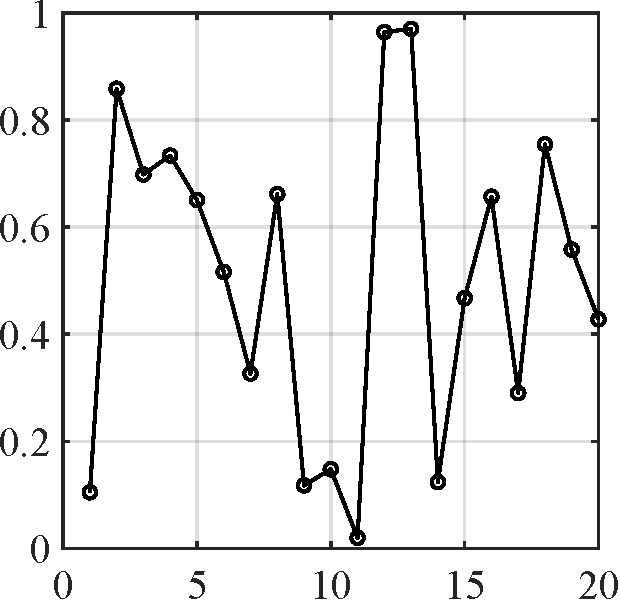
\includegraphics[height=\CE\textwidth,width=\CE\textwidth]{pic-2.pdf}}\hfill
		\subfloat[]{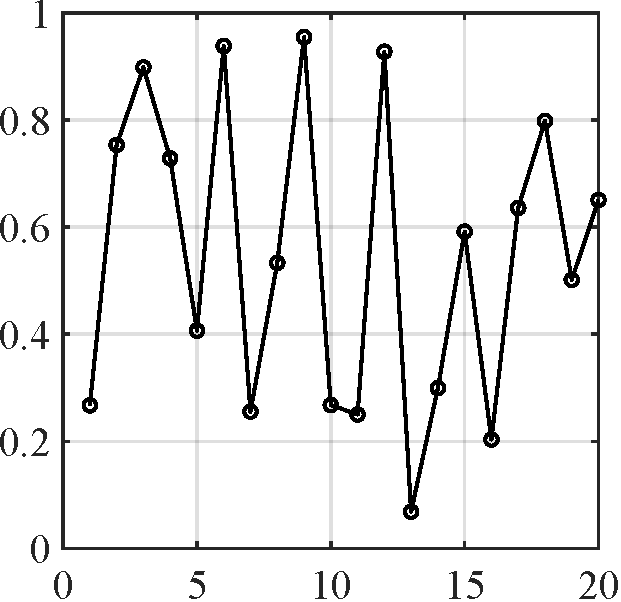
\includegraphics[height=\CE\textwidth,width=\CE\textwidth]{pic-3.pdf}}\hfill
		\subfloat[]{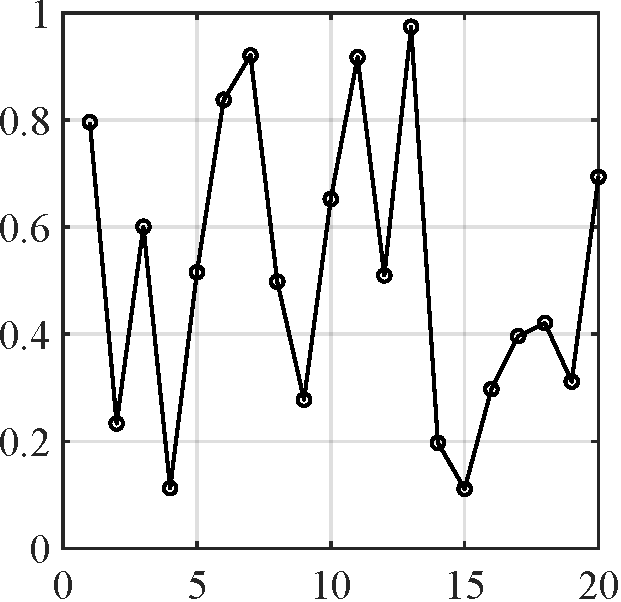
\includegraphics[height=\CE\textwidth, width=\CE\textwidth]{pic-4.pdf}}
		\captionsetup{type=figure,name=Fig.,justification=raggedright,singlelinecheck=false}
		\caption{This is a set of random data series.}
		\label{fig}
	\end{figure}
\end{document}